


\chapter{Combinatoire élémentaire}

La combinatoire est une branche importante et très belle des mathématiques. Elle se subdivise en plusieurs spécialités : combinatoire algébrique, probabiliste, analytique, arithmétique  etc.

Cette feuille est une introduction à la combinatoire élémentaire. Elle permet de faire connaissance avec les notions fondamentales en combinatoire : énumération d'objets, cardinal, permutations, partitions, coefficients binomiaux. (Dans une feuille ultérieure, on découvrira la théorie des \emph{séries génératrices}.)

%%%%%%%%%%%%%%%%%
\begin{exo}[Mains au Poker] 
Alice et Maxime jouent au Poker avec un jeu de 52 cartes (qui sont de 4 \emph{couleurs} et de 13 \emph{valeurs} possibles). 
\begin{enumerate}
\item Une \og{}main\fg{} est constituée de 5 cartes distinctes. Combien de mains y a-t-il ? 
\item Une \og{}quinte flush royale\fg{} est une suite de 5 cartes de la même couleur qui se termine par l'as: par exemple, \og{}10, valet, dame, roi, as, tous de carreau\fg{}. Combien y a-t-il de quintes flush royales ?
\item Une \og{}quinte flush\fg{} est une suite de 5 cartes de la même couleur: par exemple,  \og{}7, 8, 9, 10, valet, tous de coeur\fg{} ou \og{}as, 2, 3, 4, 5,  tous de pique\fg{}. Attention, l'as peut servir à la fois comme plus petite carte et comme plus grande carte. Combien y a-t-il de quintes flush (sans compter les quintes flush royales) ?
\item Un \og{}carré\fg{} est une main qui comporte 4 cartes de même valeur: par exemple,  \og{}les 4 rois, et le 7 de coeur\fg{}. Combien y a-t-il de carrés possibles ?
\item Un  \og{}full house\fg{} est une main qui comporte 3 cartes de même valeur (brelan), et deux autres cartes de la même valeur (paire): par exemple,  trois dames et 2 ``7''. Combien y a-t-il de full houses possibles ?
\item Un  \og{}brelan\fg{} est une main qui comporte 3 cartes de même valeur (brelan), et rien d'autre (pas de carré, pas de full house). Combien y a-t-il de brelan possibles ?
\end{enumerate}

\begin{hint} %Régine 21/03/18
Les cartes d'une main \emph{ne sont pas ordonnées}.\\
Pour la question 6: dans un jeu de 48 cartes (4 \emph{couleurs} et de 12 \emph{valeurs} possibles), combien de mains de deux cartes de valeurs différentes peut-on faire ? Attention à ne pas compter une même main plusieurs fois.
\end{hint}

\begin{sol} %Régine 21/03/18
\begin{enumerate}
\item Les cinq cartes d'une main sont distinctes et ne sont pas ordonnées: il y a donc $\binom{52}{5}=2598960$ mains possibles. 

\item Les valeurs des 5 cartes composant une quinte flush sont fixées, on peut seulement choisir la couleur: il y a donc $4$ quintes flush possibles, une par couleur. 

\item Pour compter les quintes flush non royales, on compte les valeurs possibles pour la plus petite des cartes: elle peut aller de l'as au 9 (si c'est un dix, ce sera une quinte flush, si c'est au dessus du 10, il n'y aura pas la place pour constituer une suite de 5 cartes). On a ensuite 4 choix de couleur possibles. Ca fait donc au total $9 \times 4=36$ quintes flush non royales. 

\item Comptons les carrés. On a $13$ choix pour la valeur du carré, et une fois cette valeur choisie, il nous reste à compléter la main en prenant n'importe laquelle des $48$ cartes qui ne sont pas dans le carré. On obtient donc $13\times 48=624$ carrés possibles.

\item Pour compter les full houses, on doit choisir la valeur commune pour le brelan (donc $13$) valeurs possibles, puis on doit choisir les couleurs des trois cartes du brelan (donc $4$: il suffit de choisir la couleur qu'on ne prend pas); ensuite on choisit la valeur commune pour la paire ($12$ valeurs possibles seulement, puisque l'une des valeurs est déjà prise), et finalement les couleurs des deux cartes de la paire (il y a ${4 \choose 2}=6$ façons de choisir $2$ couleurs parmi $4$ possibles. Au total, on trouve $13\times4\times 12 \times 6=3744$ full houses possibles. 

\item Pour compter les configurations de trois cartes de même valeur, on fait comme avant: $12\times 4=48$ choix possibles. Ensuite, il faut compléter avec deux cartes qui n'ont pas la même valeur entre elles, ni la même valeur que celle du brelan. On choisit donc 2 valeurs parmi les 12 disponibles (on exclut la valeur du brelan): ${12 \choose 2}=66$ choix possibles. On peut attribuer à chacun de ces cartes n'importe quelle couleur, soit $4\times 4=16$ choix de couleurs possibles pour les deux cartes complétant le brelan. Au total on trouve $48 \times 66 \times 16=50688$ brelans possibles. 
\end{enumerate}
\end{sol}
\end{exo}

%%%%%%%%%%%%%%%%%
\begin{exo}[Rangement sur l'étagère]
Alice et Maxime réorganisent leur bibliothèque qui contient $n$ livres.
\begin{enumerate}
\item Ils ne sont pas d'accord sur l'ordre dans lequel les ranger (Alice voudrait les ranger dans l'ordre chronologique de première publication alors que Maxime voudrait les classer par ordre lexicographique du corps du texte). Ils décident finalement de les ranger dans un ordre quelconque. De combien de manières peuvent-ils le faire ?
\item À la réflexion, il y a tout de même trois livres particuliers qu'ils aimeraient voir rangés côte à côte. Combien de choix ont-ils ?
\item Finalement, ils se soumettent à l'ordre moral dominant et décident de ranger ensemble les livres de chaque auteur ou autrice\footnote{Voir \url{https://www.slate.fr/story/156221/feminisation-metiers-pouvoir}.}). Leurs $n$ livres ont été écrits par $k$ auteurs (il y a $n_i$ livres du $i$-ème auteur). Combien de choix ont-ils ?
\end{enumerate}

\begin{hint} %Régine 21/03/18
On peut essayer de représenter les solutions par un arbre.  On part de la racine, et on se demande combien de possibilités on a pour la place la plus à gauche sur l'étagère: on a $n$ choix possibles, donc on fait partir $n$ branches de la racine. On va ensuite à l'extrémité de l'une de ces branches: combien de choix possibles pour la seconde place la plus à gauche ? $n-1$, donc on met $n-1$ nouvelles branches...
\end{hint}

\begin{sol} %Régine 21/03/18
\begin{enumerate}
\item Il y a $n!=n(n-1)(n-2)...\cdot 3\cdot 2\cdot 1$ ordres possibles : $n$ choix pour le premier livre, $(n-1)$ choix pour le deuxième etc.
\item On commence par placer les $(n-3)$ livres restants, il y a $(n-3)!$ choix. Ensuite, on choisit où insérer les trois livres restants, il y a $(n-2)$ emplacements possibles. Et enfin, les trois livres, même s'ils doivent être côte à côte, peuvent être rangés dans $3!=6$ ordres différents. Il y a donc $3!\cdot (n-2)!$ choix.

Une autre solution consiste à commencer par ranger les trois livres qui doivent rester ensemble entre eux: il y a $3!=6$ ordres possibles. On les considère maintenant comme un seul gros livre: on a donc $(n-3)+1=n-2$ livres à classer, donc $(n-2)!$ choix possibles. Au total $6(n-2)!$ choix possibles. 

\item Il y a $k!$ façons d'ordonner les auteurs, et ensuite, pour chaque auteur, il y a $n_i!$ façons d'ordonner les $n_i$ livres de chaque auteur. Il y a donc $k! \cdot n_1!\cdot ... \cdot n_k!$ choix au total.
\end{enumerate}
\end{sol}
% et aussi http://information.tv5monde.com/terriennes/auteure-ou-autrice-un-mot-qui-derange-23114
\end{exo}

%%%%%%%%%%%%%%%%%
\begin{exo}[Rues de New York]
Alice doit partir un an en stage à New York, ville dont les rues et avenues se croisent à angle droit à intervalles réguliers et dont le plan est assimilable à une grille. Elle doit se rendre tous les jours de son logement à son travail, ce qui correspond à aller du point de coordonnées $(0,0)$ au point $(4,5)$. Peut-elle emprunter un chemin différent tous les jours pendant un an ? (On évite les détours inutiles : on ne compte que les chemins \og de longueur $9$\fg{}.)

\begin{hint} %Régine 21/03/18
De combien de segments de rue \og vers l'est \fg{} et de combien de segments \og vers le nord \fg{} un chemin de longueur $9$ allant de $(0,0)$ à $(4,5)$ est-il composé ? 
\end{hint}

\begin{sol} %Régine 21/03/18
Un chemin est constitué de neuf segments en ligne droite, orientés vers le nord ou vers l'est. Il s'agit de choisir donc parmi les 9 segments, les quatre qui seront orientés vers l'est (et les 5 autres seront automatiquement orienté vers le nord).

Il y a donc $\binom{9}{4}$ chemins. (Ou $\binom{9}{5}$, mais c'est pareil : $\binom{n}{k} = \binom{n}{n-k}$.)

On peut calculer ce nombre avec un calculette ou par d'autres moyens, on trouve $126$, donc ça ne suffit pas à changer de chemin tous les jours pendant un an., mais ça laisse quand même pas mal de possibilités !

% autre argument en bornant par $2^8$, le neuvième choix est forcé. Et 256 est déjà trop petit !
\end{sol}
\end{exo}

%%%%%%%%%%%%%%%%%
\begin{exo}[Distribution de cadeaux]
Alice doit distribuer des bonus à certains de ses traders. Elle doit répartir $n$ cadeaux (tous identiques) à $k$ employés distincts. Combien y a-t-il de possibilités ? (Certains employés peuvent ne rien recevoir du tout et on doit distribuer l'intégralité des $n$ cadeaux.) Quel est le rapport avec l'exercice précédent ?

\begin{hint} %Régine 21/03/18
On peut essayer de représenter le problème par un chemin comme dans l'exercice précédent, en mettant en abscisse les employés numérotés de $1$ à $k$, et en ordonnée le nombre de cadeaux distribués.
\end{hint}

\begin{sol} %Régine 21/03/18
Numérotons les employés de $1$ à $k$. Pour $1 \le i \le q$, on note $f(i)$ le nombre de cadeaux donnés aux employés $1, \dots,k$. La fonction $f$ est alors une fonction croissante, de $\{1, \dots,k\}$ dans $\{0, \dots,n\}$, telle que $f(k)=n$. Si on la trace comme une fonction en escalier de $[1,k]$ dans $[0,n]$, on voit apparaître un chemin comme dans l'exercice précédent: on a un chemin de $n+k-1$ segment de longueur $1$, horizontaux ou verticaux, et il faut choisir la position des $k-1$ pas horizontaux (ou des $n$ pas verticaux). On trouve donc $\binom{n+k-1}{k-1}$ choix possibles.

Autre méthode: numérotons les employés de $1$ à $k$. Répartir $n$ objets sur les $k$ employés revient à placer $k-1$ séparateurs entre les entiers $1, 2, ..., n$ (avec éventuellement plusieurs séparateurs entre les mêmes entiers). Cela revient à se donner une liste de $n+k-1$ cases dont on doit en noircir $k-1$. Il y a donc $\binom{n+k-1}{k-1}$ choix.



%Dernière façon de compter : On veut le nombre de monômes de degré $n$ à $k$ variables. C'est une somme de coefficients multinomiaux, ceux que l'on obtient en développant $(x_1+x_2+\dots +x_k)^n$. La somme de ces coefficients multinomiaux est le résultat. Ceci est plutôt plus compliqué.
\end{sol}
\end{exo}

%%%%%%%%%%%%%%%%%
\begin{exo}[Nombre de partitions d'un entier]
Alice doit à nouveau distribuer des bonus à ses traders mais la dernière fois, ils n'étaient pas satisfaits de la distribution. Maxime lui conseille de partager les $n$~cadeaux en un certain nombre de lots et de laisser les traders se battre entre eux pour les lots. L'objectif est d'étudier le nombre de partages possibles, au niveau de la conception des lots.

En reformulant, si $n>0$, on note $p(n)$ le nombre de  façons d'écrire $n$ comme la somme d'un certain nombre d'entiers strictement positifs. (Et par convention, $p(0)=1$.) Par exemple, $p(3)=3$ car on peut décomposer $3$ de trois façons différentes : $3$, $2+1$ et $1+1+1$. On peut représenter un partage avec un diagramme (diagramme de Ferrers)

\begin{figure}[h!]
\begin{center}
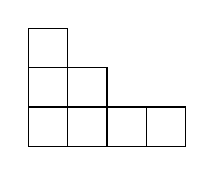
\begin{tikzpicture}[scale=0.5]
(0,2) rectangle (2,0);
%(0,0) rectangle (4,1);
\draw (0,0)  -- (4,0)  -- (4,1) -- (0,1) -- cycle;
\draw (0,1)  -- (2,1)  -- (2,2) -- (0,2) -- cycle;
\draw (0,0)  -- (1,0)  -- (1,3) -- (0,3) -- cycle;
\draw (2,0)  -- (3,0)  -- (3,1) -- (2,1) -- cycle;
%(0,1) rectangle (2,2);
%(0,0) rectangle (1,3);
\end{tikzpicture}
\caption{représentation de $\{3,2,1,1\}$, un  partage de l'entier $7$ en $4$ parts}
\end{center}
\end{figure}




\begin{enumerate}
\item Calculer $p(n)$ pour $n\leq 6$.% 1, 2, 3, 5, 7, 11
\item Notons $p_k(n)$, le nombre de partages de l'entier $n$ en $k$ parts non nulles. Montrer la formule $p_k(n)=p_{k-1}(n-1)+p_k(n-k)$.
En déduire que l'on peut calculer les $p(n)$ de proche en proche. 
\end{enumerate}
On reviendra sur cet exercice dans une prochaine feuille, en utilisant des séries génératrices.

\begin{hint} %Régine 21/03/18
Partitionner les partages en $k$ parts de l'entier $n$ entre ceux qui contiennent des parts égales à $1$ et ceux qui n'en contiennent pas. 
Faire des diagrammes de Ferrers. 
\end{hint}

\begin{sol} %Régine 21/03/18
\begin{enumerate}
\item La suite commence par 1, 2, 3, 5, 7, 11, 15, 22
\item Partitionnons les partages en $k$ parts de l'entier $n$ entre ceux qui contiennent des parts égales à $1$ et ceux qui n'en contiennent pas. Dans le diagramme de Ferrers d'un partage ne contenant pas de part égale à $1$, si on efface la ligne du bas du diagramme, on obtient un partage de $n-k$ en $k$ parts. Dans le diagramme de Ferrers d'un partage contenant au moins une part égale à $1$, si on efface la part égale à $1$ la plus à droite, on obtient un partage de $n-1$ en $k-1$ parts. Ainsi, $p_k(n)=p_{k-1}(n-1)+p_k(n-k)$.
\end{enumerate}
\end{sol}
\end{exo}

%%%%%%%%%%%%%%%%%
\begin{exo}[Collier de perles]
Maxime veut offrir un collier à Alice. Il peut acheter des perles de deux couleurs différentes, dans la quantité souhaitée. Combien de colliers vraiment différents à $n$ perles peut-il concevoir ? (Le fermoir doit être placé derrière le cou, mais on peut retourner le collier pour le porter \og dans l'autre sens\fg.)


Note : si on peut de plus faire \og tourner\fg{} le collier (par exemple si le fermoir est invisible), l'exercice devient vraiment difficile et nécessite des connaissances d'arithmétique (groupes cycliques et indicatrice d'Euler). Dans une prochaine feuille !

\begin{hint} %Régine 21/03/18
Combien peut-on écrire de mots de $n$ lettres avec l'alphabet $\{a,b\}$ ? Combien peut-on écrire de mots palindromes de $n$ lettres avec l'alphabet $\{a,b\}$ ? on pourra traiter séparément le cas $n$ pair et $n$ impair.
\end{hint} 

\begin{sol} %Régine 21/03/18
Si on ne compte pas la symétrie consistant à retourner le collier, il y a $2^n$ colliers possibles. Parmi ceux-là, certains sont symétriques, d'autre pas.

Rappel: on note $\lceil x \rceil$ l'entier $n$ tel que $n-1<x \le n$.

Pour concevoir un collier symétrique, on doit choisir $\lceil n/2 \rceil$ perles : les perles restantes ont une couleur déterminée par la symétrie. Il y a donc $2^{\lceil n/2 \rceil}$ colliers symétriques, les autres, au nombre de $2^n - 2^{\lceil n/2 \rceil}$, ne le sont pas, et peuvent être donc classés par paires (deux colliers symétriques l'un par rapport à l'autre. Chacune de ces paires de colliers constitue en fait un seul \og type\fg{} de collier.

Il y a donc 
\[ 2^{\lceil n/2 \rceil} + \frac{2^n-2^{\lceil n/2 \rceil}}{2} = \frac{2^n+2^{\lceil n/2 \rceil}}{2}\]
types de colliers.

Par exemple, il y a $20$ types de colliers à cinq perles.

L'exercice devient bien plus difficile si l'on autorise les rotations du collier. Le cadre général est celui du comptage du nombre d'orbites dans une action de groupe, en général à l'aide de la formule de Burnside.
\end{sol}
\end{exo}

%%%%%%%%%%%%%%%%%
\begin{exo}[Plan de table]
Alice et Maxime se marient. Tous les convives, au nombre de $n$, seront placés autour d'une grande table circulaire.
\begin{enumerate}
\item Combien de plans de table sont possibles ? On considère que si l'on fait tourner la table (ou les convives), cela ne change rien, mais que par contre la droite et la gauche ne sont pas interchangeables. 
\item Et si Alice et Maxime doivent être placés côte à côte ?
\item Et si on veut alterner filles et garçons (en supposant que  ce soit possible) ?
\end{enumerate}

\begin{hint} %Régine 21/03/18
Comme on peut faire tourner la table, on peut dire qu'on place Alice à la place $1$, et numéroter les places restantes de $2$ à $n$ dans le sens des aiguilles d'une montre. 
\end{hint}

\begin{sol} %Régine 21/03/18
\begin{enumerate}
\item On commence par placer Alice. On pourrait dire qu'elle a $n$ places possibles, mais faire tourner la table ne change rien: on considère donc qu'on la place sur la place numéro 1. On numérote ensuite les $n-1$ places restantes de $2$ à $n$, dans le sens des aiguilles d'une montre. Il nous reste à placer $n-1$ convives sur $n-1$ places, donc $(n-1)!$.
\item On place Alice et Maxime sur les places $1$ et $2$ (et il y a deux façons possibles) puis on place les $n-2$ convives restants sur $n-2$ places restantes, donc $2 \cdot (n-2)!$.
\item On suppose donc que $n=2k$ est pair et qu'il y a $k$ filles et $k$ garçons. On imagine qu'on fait une table de $k$ filles avec Alice à la place $1$: il y a $(k-1)!$ choix possibles. On fait aussi une table de $k$ garçons avec Maxime à la place $1$: il y a aussi $(k-1)!$ choix possibles. Il nous reste à intercaler les deux tables, ce qu'on peut faire de $k$ manières possibles. Donc au final, $k\cdot (k-1)!^2$ plans de table possibles.
\end{enumerate}
\end{sol}
\end{exo}

%%%%%%%%%%%%%%%%%
\begin{exo}[Partitions d'un ensemble]
Alice et Maxime cherchent à faire la place dans leur appartement (voir exercice suivant) en donnant des livres à leurs amis. Ils ont $n$ livres (tous différents) à donner et décident de faire des lots que leurs amis (tous différents...) se partageront comme ils le voudront. Combien y a-t-il de manières de concevoir les lots ?

En reformulant, si $X$ est un ensemble de cardinal $n$, on cherche le nombre $B(n)$ de partitions de cet ensemble (en parties non vides). 

\begin{enumerate}
\item Calculer $B(n)$ pour $n\leq 5$.
\item Montrer la relation d'Aitken
\[B_{n+1} = \sum_{k=0}^{n} \binom{k}{n}B_k.  \]
\end{enumerate}

\begin{hint} %Régine 21/03/18
Trier les partitions de $\{1, \dots, n+1\}$ en fonction du nombre d'éléments qui ne sont pas dans la même partie que $n+1$.
\end{hint}

\begin{sol} %Régine 21/03/18
\begin{enumerate}
\item La suite des nombres de Bell commence par:1, 1, 2, 5, 15, 52, 203...
\item On trie les partitions de $\{1, \dots, n+1\}$ en fonction du nombre $k$ d'éléments qui ne sont pas dans la même partie que $n+1$: ce cardinal varie de $0$ à $n$. On commence par choisir les $k$ éléments de $\{1, \dots,n\}$ qui ne sont pas dans la même partie que $n+1$: il y a ${n \choose k}$ façons de le faire, puis on choisit une partition de cette partie à $k$ éléments, et il y en a $B(k)$. Donc au final, 
\[B_{n+1} = \sum_{k=0}^{n} \binom{k}{n}B_k.  \]

\end{enumerate}
\end{sol}
\end{exo}


%%%%%%%%%%%%%%%%%
\begin{exo}[Anagrammes]
Alice et Maxime choisissent un prénom pour leur premier enfant.

Ils décident d'utiliser exactement les lettres  suivantes : a, e, g, i, l, l, m, u, u.  Combien d'anagrammes y a-t-il sur ces neuf lettres ?

(Note : on peut reformuler la réponse en termes de \emph{coefficients multinomiaux}, des généralisations des coefficients binomiaux.)

\begin{hint} %Régine 21/03/18
Combien d'anagrammes peut-on former à partir de $9$ lettres deux à deux distinctes ? Quelle est le problème quand une même lettre apparaît plusieurs fois ? 
\end{hint}

\begin{sol} %Régine 21/03/18

\paragraph{Première méthode.} 
On place les deux \og{}l\fg{}, il y a $\binom{9}{2}$ choix. Ensuite, on place les deux \og{}u\fg{}, il y a $\binom{7}{2}$ choix. Puis on place les cinq lettres qui restent : $5!$ choix. Finalement, on a $\binom{9}{2}\cdot\binom{7}{2}\cdot 5!=90720$.


\paragraph{Deuxième méthode.} 
Si on distingue les deux \og{}l\fg{} et les deux \og{}u\fg{} en les coloriant en bleu et rouge par exemple, on a donc neuf lettres distinctes. Il y a $9!$ mots possibles avec ces neuf lettres.

Si on veut oublier la distinction, on voit que chaque mot est compté quatre fois avec la première méthode de comptage. Par exemple, \og Guillaume\fg{} est compté quatre fois de la façon suivante:
\begin{enumerate}
\item G{\bf\color{red}u}i{\bf\color{red}l}{\bf\color{blue}l}a{\bf\color{blue}u}me
\item G{\bf\color{blue}u}i{\bf\color{red}l}{\bf\color{blue}l}a{\bf\color{red}u}me
\item G{\bf\color{red}u}i{\bf\color{blue}l}{\bf\color{red}l}a{\bf\color{blue}u}me
\item G{\bf\color{blue}u}i{\bf\color{blue}l}{\bf\color{red}l}a{\bf\color{red}u}me
\end{enumerate}

On divise donc $9!$ par quatre, ce qui redonne bien le résultat trouvé précédemment : $9!/4 = 90720$.


\paragraph{Ce qu'il y a derrière :  coefficients multinomiaux} La deuxième méthode fait penser au calcul des coefficients binomiaux avec les factorielles. En filigrane, il y a les coefficients multinomiaux, des généralisations des coefficients binomiaux, qui servent exactement à compter les anagrammes. Voire par exemple \url{https://fr.wikipedia.org/wiki/Formule_du_multin%C3%B4me_de_Newton}
 et \url{https://fr.wikipedia.org/wiki/Permutation_avec_r%C3%A9p%C3%A9tition}
\end{sol}
\end{exo}






%%%%%%%%%%%%%%%%%
\begin{exo}[Nombres de Catalan]
% pour les puissances successives, aussi : a^b^c^d.
Maxime apprend la division à l'ENS. Enthousiasmé, il essaye de faire plusieurs divisions de suite et écrit \og $ a\div b \div c$ \fg. Son professeur Cédric Villani lui fait remarquer que cette expression n'est pas bien définie : elle peut signifier \og$(a\div b)\div c$ \fg, ou bien \og $a\div (b\div c)$ \fg{} et le résultat peut varier suivant l'ordre de priorité choisi pour effectuer les divisions. (En langage savant, on dit que la division n'est pas \emph{associative} : les divisions successives doivent être parenthésées pour avoir un sens.)

Au lieu de finir l'exo, Maxime se demande alors de combien de façons on peut parenthéser une suite ordonnée de symboles \og$a_0~a_1~\dots ~ a_n$\fg. Ce nombre de parenthésages est noté $C_n$ dans la suite. On a vu que $C_2 = 2$, en effet la suite ordonnée de symboles \og $a_0~a_1~a_2$\fg{} peut être parenthésée de deux façons : $(a_0a_1)a_2$ ou bien $a_0(a_1a_2)$.

\begin{enumerate}
\item Montrer que $C_3 = 5$, et calculer $C_4$.
\item Trouver une formule de récurrence permettant de calculer les nombres $C_n$.
\end{enumerate} 

\begin{sol} %Régine 21/03/18: ouh la la il est trop dur cet exercice !
$C_4=14$ et $C_5=42$.

Formule de récurrence $C_{n+1} = \sum_{k=0}^n C_kC_{n-k}$.

Il existe une formule close : 
\[ C_n = \binom{2n}{n} - \binom{2n}{n+1}\]
(Tous les mots, moins les mots qui ne sont pas de Dyck.)
\end{sol}
\end{exo}

Les thèmes abordés dans cette feuille sont les suivants : nombre de partitions d'un entier, nombres de Bell, nombres de Catalan. Sur les nombres de Catalan, on conseille la vidéo suivante : \url{https://www.youtube.com/watch?v=aqQjrHeHXP4} (qui va assez loin : certains de ces points seront développés dans des séances ultérieures).\\
